\section{The file format}
\label{sec:format}

A WSQ file is a sequence of bytes organized like a JPEG file (Annex B). It is made of
\emph{markers}, two-byte codes \hex{FF} followed by a byte other than \hex{00} and \hex{FF};
of \emph{marker segments}, a marker followed by a 16-bit length and a list of parameters; and
of \emph{entropy-coded segments} (ECS), the Huffman-coded data. Multi-byte parameters are
big-endian. The length of a marker segment counts its own two bytes and the parameters, but
not the marker. Any marker may be preceded by any number of \hex{FF} fill bytes.
Table~\ref{tab:markers} lists the markers.

\begin{table}[ht]
  \centering\small
  \begin{tabular}{@{}lll@{}}
    \toprule
    code & name & meaning \\
    \midrule
    \hex{FFA0} & \marker{SOI} & start of image (no segment) \\
    \hex{FFA1} & \marker{EOI} & end of image (no segment) \\
    \hex{FFA2} & \marker{SOF} & start of frame: the frame header \\
    \hex{FFA3} & \marker{SOB} & start of block: the block header \\
    \hex{FFA4} & \marker{DTT} & define transform table (the wavelet filters) \\
    \hex{FFA5} & \marker{DQT} & define quantization table \\
    \hex{FFA6} & \marker{DHT} & define Huffman table(s) \\
    \hex{FFA7} & \marker{DRI} & define restart interval \\
    \hex{FFA8} & \marker{COM} & comment \\
    \hex{FFB0}--\hex{FFB7} & \marker{RST}$_m$ & restart marker, $m = 0..7$ cyclically (no segment) \\
    \bottomrule
  \end{tabular}
  \caption{Marker codes (Table B.1 of the specification).}
  \label{tab:markers}
\end{table}

\subsection{Structure}

A file is \marker{SOI}, one \emph{frame}, \marker{EOI}. The frame is a frame header followed by
one or more blocks; each block is a block header followed by its entropy-coded data. Table and
comment segments may come before the frame header and before any block header. When a table is
defined more than once, the latest definition replaces the earlier ones. Figure~\ref{fig:stream}
shows a file written by the NIST encoder; its segments have lengths 124 (\marker{COM}),
58 (\marker{DTT}), 389 (\marker{DQT}), 17 (\marker{SOF}), 193 and 149 (the two \marker{DHT}) and
3 (each \marker{SOB}).

\begin{figure}[ht]
  \centering
  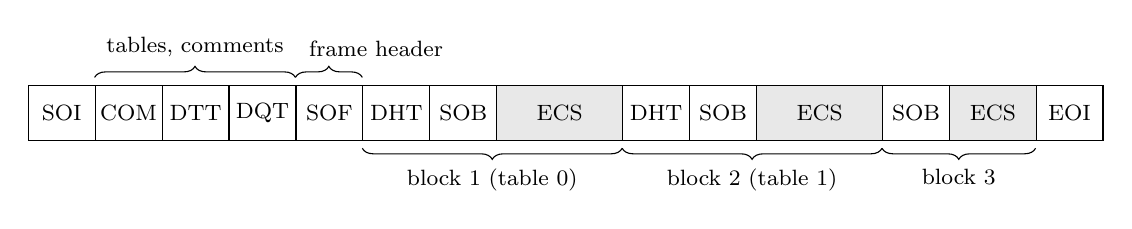
\begin{tikzpicture}[x=1cm,y=1cm,font=\footnotesize,
    seg/.style={draw,minimum height=7mm,inner sep=1pt,anchor=west},
    ecs/.style={seg,fill=gray!18}]
  \def\row#1{%
    \foreach \name/\w/\st [remember=\x as \lastx (initially 0)] in {#1} {
      \pgfmathsetmacro{\x}{\lastx+\w}
      \node[\st,minimum width=\w cm] at (\lastx,0) {\name};
    }}
  \begin{scope}
    \row{\marker{SOI}/0.85/seg, \marker{COM}/0.85/seg, \marker{DTT}/0.85/seg, \marker{DQT}/0.85/seg,
         \marker{SOF}/0.85/seg, \marker{DHT}/0.85/seg, \marker{SOB}/0.85/seg, ECS/1.6/ecs,
         \marker{DHT}/0.85/seg, \marker{SOB}/0.85/seg, ECS/1.6/ecs,
         \marker{SOB}/0.85/seg, ECS/1.1/ecs, \marker{EOI}/0.85/seg}
  \end{scope}
  \draw[decorate,decoration={brace,amplitude=4pt}] (0.85,0.45) -- (3.4,0.45)
    node[midway,above=4pt] {tables, comments};
  \draw[decorate,decoration={brace,amplitude=4pt}] (3.4,0.45) -- (4.25,0.45)
    node[midway,above=4pt,xshift=6mm] {frame header};
  \draw[decorate,decoration={brace,amplitude=4pt,mirror}] (4.25,-0.45) -- (7.55,-0.45)
    node[midway,below=4pt] {block 1 (table 0)};
  \draw[decorate,decoration={brace,amplitude=4pt,mirror}] (7.55,-0.45) -- (10.85,-0.45)
    node[midway,below=4pt] {block 2 (table 1)};
  \draw[decorate,decoration={brace,amplitude=4pt,mirror}] (10.85,-0.45) -- (12.8,-0.45)
    node[midway,below=4pt] {block 3};
\end{tikzpicture}

  \caption{Layout of a file written by the NIST encoder. Shaded boxes are entropy-coded data.}
  \label{fig:stream}
\end{figure}

The specification also defines two \emph{abbreviated formats}: compressed image data with some
or all tables omitted, to be decoded with tables installed earlier, and a file with tables but
no frame, used only to install tables (\marker{SOI}, tables, \marker{EOI}). In the ordinary
\emph{interchange format} every table needed to decode the image is present.

\subsection{Scaled integers}
\label{sec:scaled}

Real-valued parameters (the normalization constants, the filter taps, the bin widths) are
stored as a pair: an 8-bit exponent $E$ and an unsigned integer $V$ of 16 or 32 bits, meaning
$V/10^E$. The specification does not say how to choose $E$. The NIST encoder takes the largest
$E$ for which the rounded $V$ still fits, which keeps four to five significant digits for 16-bit
values and nine to ten for 32-bit ones: starting from the value, it multiplies by 10 until the
result reaches the largest unsigned value ($65535$ or $2^{32}-1$), steps back once, and rounds.
Zero is stored as $E = 0$, $V = 0$. Signs, where needed, travel in a separate byte.

\subsection{Segments}

Tables~\ref{tab:sof} to~\ref{tab:dht} give the layout of each segment, field by field, with
the sizes in bits and the values the NIST encoder writes.

\begin{table}[ht]
  \centering\small
  \begin{tabular}{@{}llp{9.3cm}@{}}
    \toprule
    field & bits & meaning \\
    \midrule
    $L_f$ & 16 & segment length, 17 \\
    $A$ & 8 & scanner black calibration value (0) \\
    $B$ & 8 & scanner white calibration value (255) \\
    $Y$ & 16 & number of lines (image height) \\
    $X$ & 16 & samples per line (image width) \\
    $E_m$, $M$ & 8, 16 & normalization shift $M$ as a scaled integer \\
    $E_r$, $R$ & 8, 16 & normalization scale $R$ as a scaled integer \\
    $E_v$ & 8 & encoder number: 2 for encoder number two (the value version 3.1 introduced) \\
    $S_f$ & 16 & software implementation number (0) \\
    \bottomrule
  \end{tabular}
  \caption{Frame header (\marker{SOF}, Figure B.3).}
  \label{tab:sof}
\end{table}

\begin{table}[ht]
  \centering\small
  \begin{tabular}{@{}llp{9.3cm}@{}}
    \toprule
    field & bits & meaning \\
    \midrule
    \multicolumn{3}{@{}l}{\textit{Block header} (\marker{SOB}, Figure B.4)}\\
    $L_s$ & 16 & segment length, 3 \\
    $T_d$ & 8 & Huffman table used by this block, 0 to 7 \\
    \midrule
    \multicolumn{3}{@{}l}{\textit{Transform table} (\marker{DTT}, Figure B.6)}\\
    $L_t$ & 16 & segment length (58 for the 9/7 bank) \\
    $L_0$, $L_1$ & 8, 8 & lengths of $h_0$ and $h_1$ \\
    $S_n$, $E_x$, $H$ & 8, 8, 32 & for each transmitted tap, first of $h_0$ then of $h_1$, starting at the
      centre: sign (nonzero means negative), exponent and magnitude; $\ceil{L_i/2}$ taps per filter \\
    \midrule
    \multicolumn{3}{@{}l}{\textit{Quantization table} (\marker{DQT}, Figure B.7)}\\
    $L_q$ & 16 & segment length, 389 \\
    $E_c$, $C$ & 8, 16 & bin centre parameter $C$ (encoder number two: $E_c = 2$, $C = 44$) \\
    $E_q$, $Q_k$, $E_z$, $Z_k$ & 8, 16, 8, 16 & for $k = 0..63$: bin width and zero-bin width \\
    \midrule
    \multicolumn{3}{@{}l}{\textit{Restart interval} (\marker{DRI}, Figure B.9)}\\
    $L_r$ & 16 & segment length, 4 \\
    $R_i$ & 16 & coefficients per restart interval; 0 disables restarts \\
    \midrule
    \multicolumn{3}{@{}l}{\textit{Comment} (\marker{COM}, Figure B.10)}\\
    $L_c$ & 16 & segment length \\
    $C_m$ & $8(L_c-2)$ & comment bytes, interpreted by the application \\
    \bottomrule
  \end{tabular}
  \caption{Block header and table segments.}
  \label{tab:segments}
\end{table}

\begin{table}[ht]
  \centering\small
  \begin{tabular}{@{}llp{9.3cm}@{}}
    \toprule
    field & bits & meaning \\
    \midrule
    $L_h$ & 16 & segment length \\
    \multicolumn{3}{@{}l}{\textit{then, for each table, until the segment ends:}}\\
    $T_h$ & 8 & table number, 0 to 7 \\
    $L_1,\dots,L_{16}$ & $16\times 8$ & $\mathrm{BITS}$: number of codes of each length \\
    $V_{i,j}$ & $8\sum_i L_i$ & $\mathrm{HUFFVAL}$: the symbols, by increasing code length \\
    \bottomrule
  \end{tabular}
  \caption{Huffman table segment (\marker{DHT}, Figure B.8). One segment may define several
  tables; the NIST encoder writes one segment per table.}
  \label{tab:dht}
\end{table}

\subsection{Restart intervals}

If a \marker{DRI} segment sets a nonzero interval $R_i$, the encoder ends an entropy-coded
segment after every $R_i$ coefficients and writes a restart marker, cycling through
\marker{RST}$_0$ to \marker{RST}$_7$; the decoder can then resynchronize after an error. The
bit buffer is padded and flushed at each restart. Restarts are optional and the NIST encoder
never uses them.

\subsection{Resolution and the NISTCOM comment}

The frame header carries no resolution. In ANSI/NIST-ITL transactions the resolution is a field
of the record that contains the WSQ data. Standalone files written by the NIST tools carry it in
a comment segment that begins with the text \texttt{NIST\_COM} and continues with
\texttt{KEY value} lines, for example
\begin{center}\small
\texttt{NIST\_COM 9 \quad PIX\_WIDTH 1452 \quad PIX\_HEIGHT 1006 \quad PIX\_DEPTH 8 \quad PPI 500}\\
\texttt{LOSSY 1 \quad COLORSPACE GRAY \quad COMPRESSION WSQ \quad WSQ\_BITRATE 0.750000}
\end{center}
This \emph{NISTCOM} convention comes from NBIS, not from the WSQ specification, but readers
commonly rely on it.

\subsection{Parsing}

Algorithm~\ref{alg:parse} reads a file. Each table segment updates the decoder state; each block
header starts an entropy-coded segment, which ends at the first marker that is not a restart
marker.

\begin{algorithm}[ht]
  \caption{Reading a WSQ file.}
  \label{alg:parse}
  \begin{algorithmic}[1]
    \Require the bytes of a file
    \Ensure frame parameters, tables, and a list of blocks (table number, entropy-coded bytes)
    \Function{ReadMarker}{}
      \State require byte \hex{FF}; skip further \hex{FF} bytes; \Return \hex{FF00} $+$ next byte
    \EndFunction
    \State require \Call{ReadMarker}{} $=$ \marker{SOI}
    \Loop
      \State $m \gets \Call{ReadMarker}{}$
      \If{$m = \marker{EOI}$} \textbf{break} \EndIf
      \State $L \gets$ 16-bit length;\ the segment ends $L$ bytes after the length field starts
      \If{$m = \marker{DTT}$} read $L_0$, $L_1$ and the taps; expand $h_0, h_1$; derive $f_0, f_1$ by Eq.~\eqref{eq:antialias}
      \ElsIf{$m = \marker{DQT}$} read $C$ and $Q_k$, $Z_k$ for $k = 0..63$
      \ElsIf{$m = \marker{DHT}$} read tables until the segment ends; build them with Algorithm~\ref{alg:codes}
      \ElsIf{$m = \marker{DRI}$} read $R_i$
      \ElsIf{$m = \marker{COM}$} keep the bytes (look for \texttt{NIST\_COM} and \texttt{PPI})
      \ElsIf{$m = \marker{SOF}$} read $Y$, $X$, $M$, $R$, $E_v$
      \ElsIf{$m = \marker{SOB}$}
        \State read $T_d$; collect bytes up to the next marker other than \marker{RST}$_m$,
               replacing each \hex{FF}\,\hex{00} pair by \hex{FF}; record the block
      \Else\ \textbf{fail}: unknown marker
      \EndIf
    \EndLoop
  \end{algorithmic}
\end{algorithm}
